\documentclass[12pt]{article}
\usepackage{graphicx}
\usepackage{amsfonts}
\usepackage{fancyhdr}
\usepackage{comment}
\usepackage{amsmath}
\usepackage[a4paper, top=2.5cm, bottom=2.5cm, left=2.2cm, right=2.2cm]%
{geometry}
\usepackage{times}
\usepackage{amsmath}
\usepackage{changepage}
\usepackage{amssymb}
\usepackage{fixltx2e}
\usepackage{enumerate}
\usepackage{graphicx}
\usepackage{float}
\newtheorem{theorem}{Theorem}
\newtheorem{acknowledgement}[theorem]{Acknowledgement}
\newtheorem{algorithm}[theorem]{Algorithm}
\newtheorem{axiom}{Axiom}
\newtheorem{case}[theorem]{Case}
\newtheorem{claim}[theorem]{Claim}
\newtheorem{conclusion}[theorem]{Conclusion}
\newtheorem{condition}[theorem]{Condition}
\newtheorem{conjecture}[theorem]{Conjecture}
\newtheorem{corollary}[theorem]{Corollary}
\newtheorem{criterion}[theorem]{Criterion}
\newtheorem{definition}[theorem]{Definition}
\newtheorem{example}[theorem]{Example}
\newtheorem{exercise}[theorem]{Exercise}
\newtheorem{lemma}[theorem]{Lemma}
\newtheorem{notation}[theorem]{Notation}
\newtheorem{problem}[theorem]{Problem}
\newtheorem{proposition}[theorem]{Proposition}
\newtheorem{remark}[theorem]{Remark}
\newtheorem{solution}[theorem]{Solution}
\newtheorem{summary}[theorem]{Summary}
\newenvironment{proof}[1][Proof]{\textbf{#1.} }{\ \rule{0.5em}{0.5em}}

\newcommand{\Q}{\mathbb{Q}}
\newcommand{\R}{\mathbb{R}}
\newcommand{\C}{\mathbb{C}}
\newcommand{\Z}{\mathbb{Z}}

\begin{document}

\title{SIE 545: Fundamentals of Optimization \\Homework 4}
\author{Martin Manuel Lopez \\lopez9@email.arizona.edu \\Systems and Industrial Engineering}
\date{November 11, 2018}
\maketitle
\section{BSS 4.2}   
    \begin{align*}
        &max \quad x_1+3x_2 \\
        &\text{s.t} \\
        &2x_1 + 3x_2 \leq 6\\
        &-x_1 + 4x_2 \leq 4\\
        &x_1 \geq 0\\
        &x_2 \geq 0\\
    \end{align*}
    \text{We reformulate the problem and utilize the dual to find the minimization of problem:}\\
    \begin{align*}
        &min -x_1 - 3x_2\\
        &\text{s.t.}\\
        &-2x_1-3x_2 \geq 6\\
        &x_1 -4x_2 \geq 4\\
        &-x_1 \leq 0 \\
        &-x_2 \leq 0\\
    \end{align*}
Graphically we can demonstrate the feasible region based on the constraints and the objective function\\
    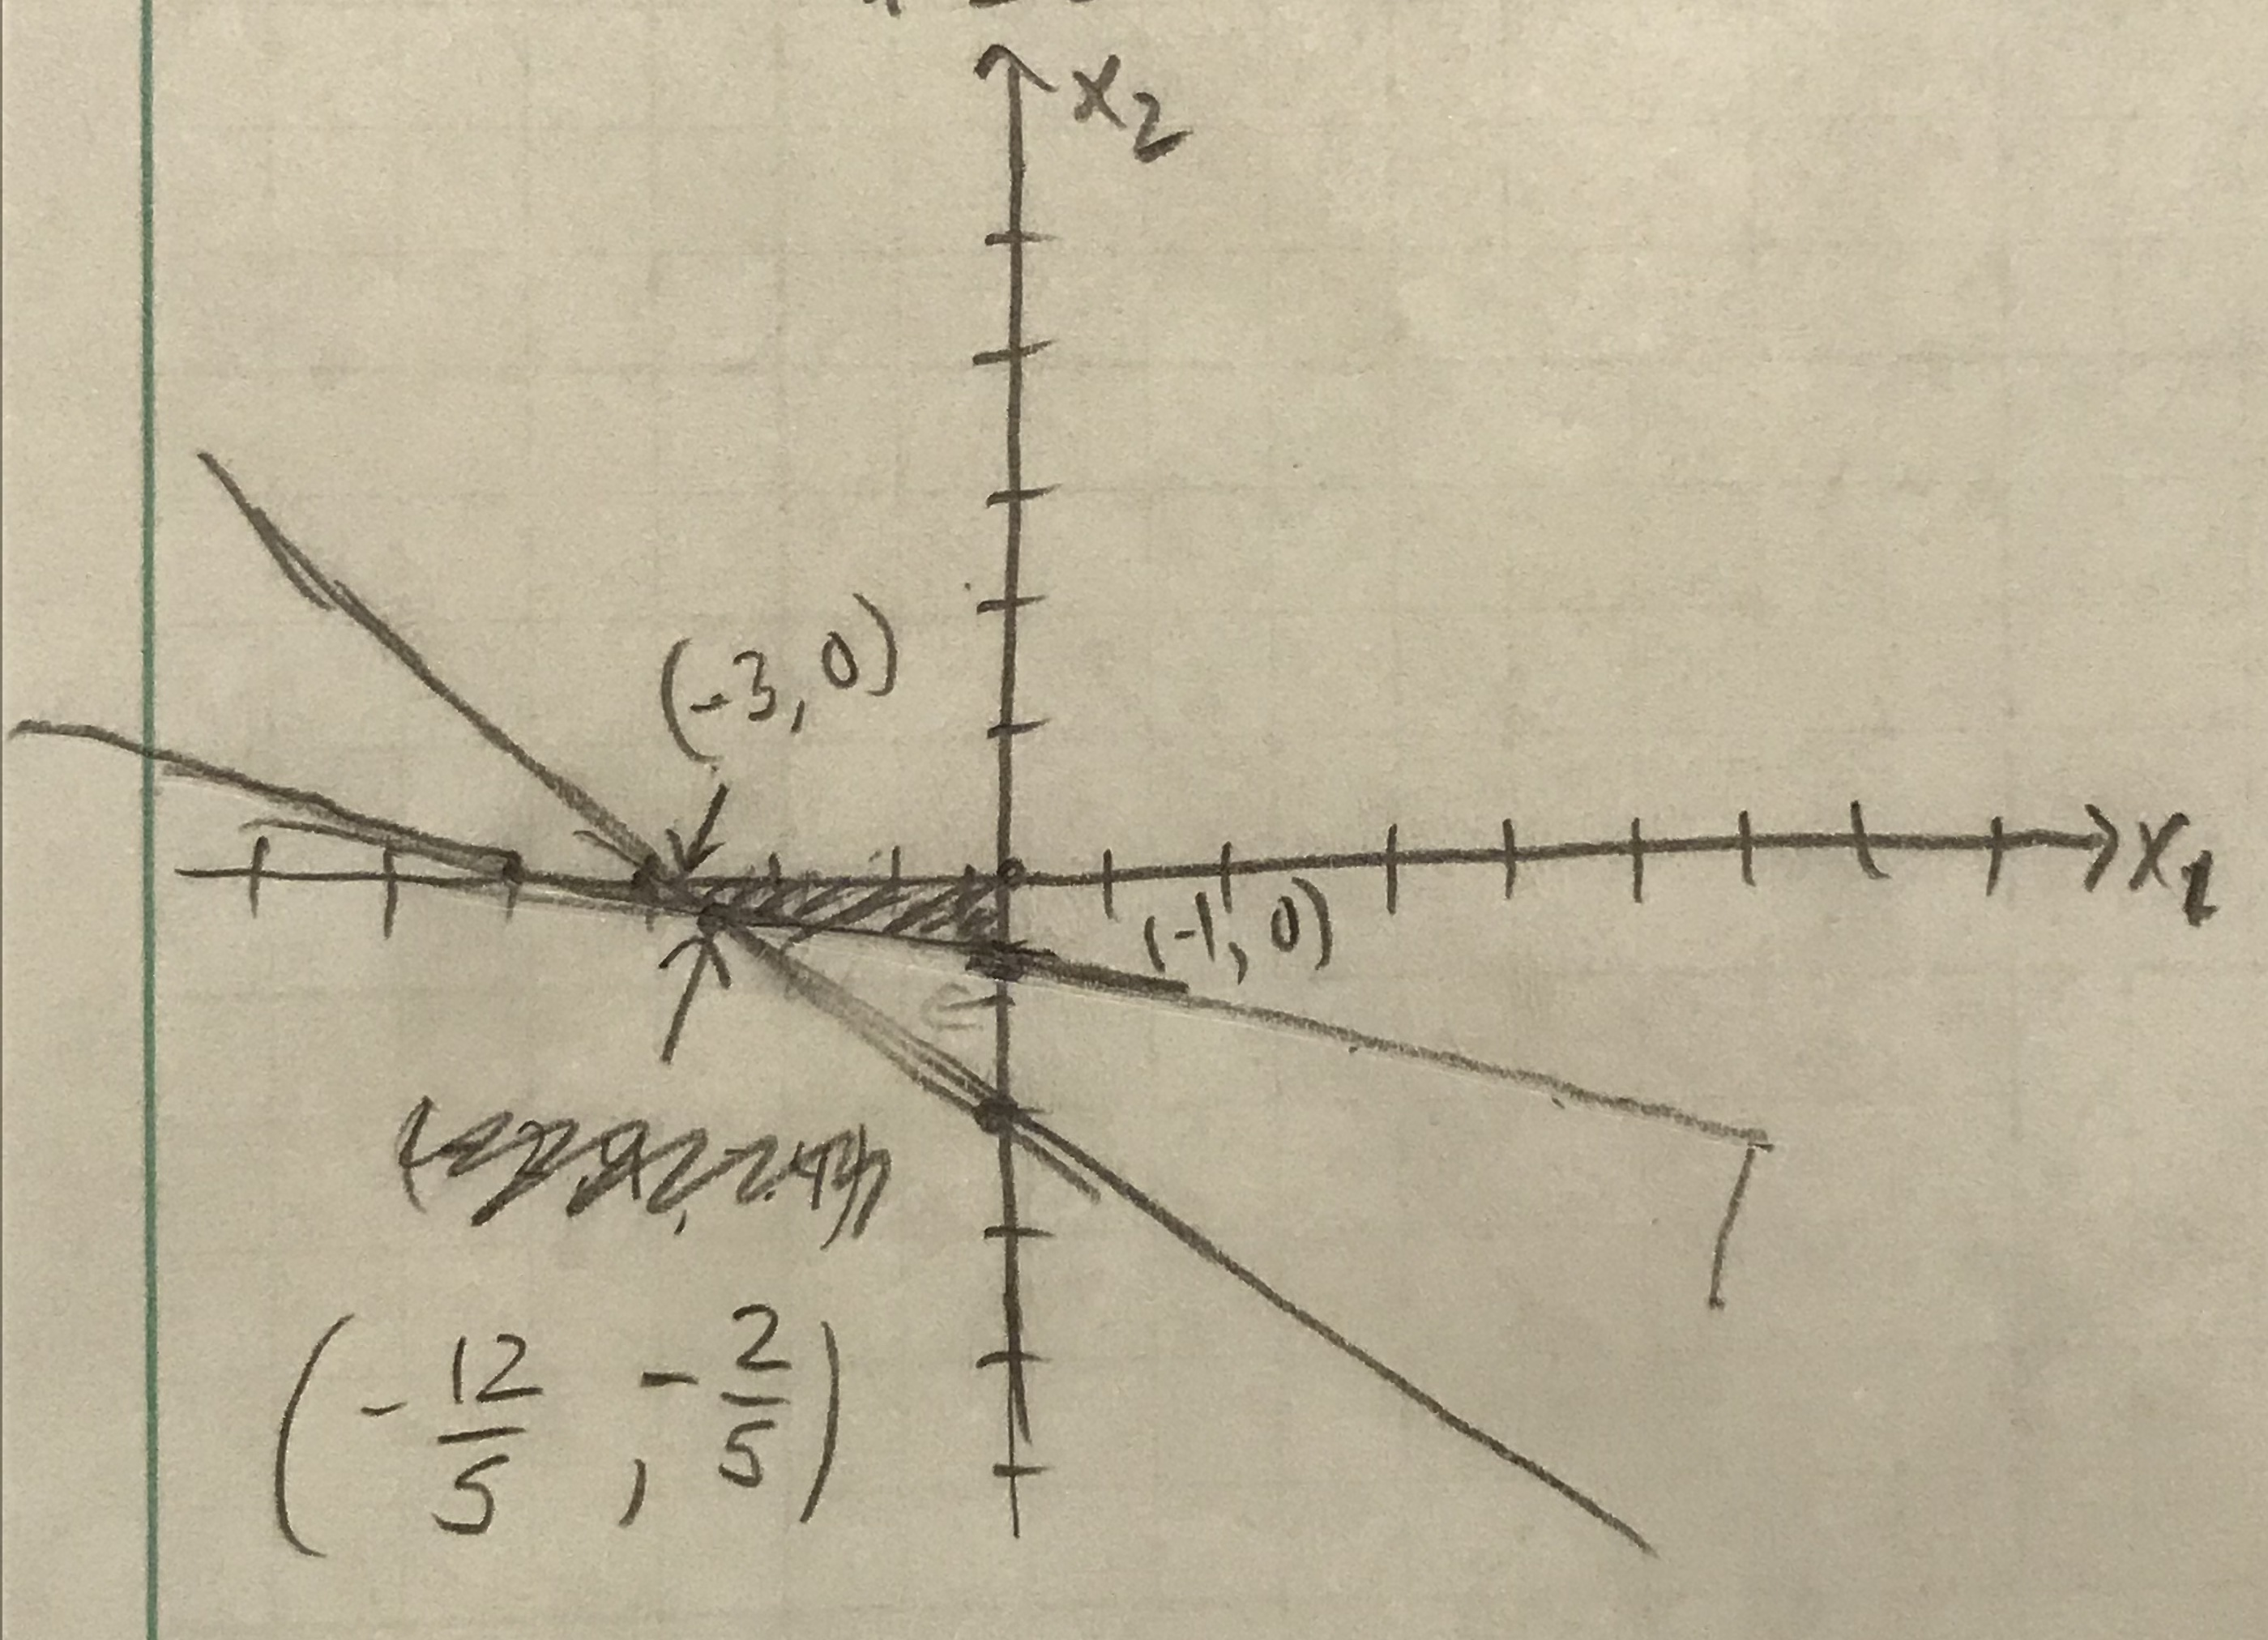
\includegraphics[width=\textwidth]{BSS4-2.jpeg}\\
    \text{a.) Based on the KKT conditions we have the following: }\\
    \begin{align*}
        &\nabla f(\bar x) + \sum_{i \in I} u_i \nabla g_i(\bar x) = 0
    \end{align*}
    We determine the following gradient and active constraints to determine which KKT optimality conditions for the extreme points\\
    \begin{align*}
        &\nabla f(\bar x) = 
            \begin{bmatrix}
                -1\\
                -3\\
            \end{bmatrix}\\
        &\nabla g_1(\bar x) = 
            \begin{bmatrix}
                -2\\
                -3\\
            \end{bmatrix}\\
        &\nabla g_2(\bar x) = 
            \begin{bmatrix}
                -1\\
                -4\\
            \end{bmatrix}\\
        &\nabla g_3(\bar x) = 
            \begin{bmatrix}
                -1\\
                0\\
            \end{bmatrix}\\
        &\nabla g_4(\bar x) = 
            \begin{bmatrix}
                0\\
                -1\\
            \end{bmatrix}\\
    \end{align*}
    b.) Now we write the optimality conditions for extreme point (-3,0)\\
    \begin{align*}
        &u_0 (-1,-3)^T + u_1 (-2,-3)^T + u_2 (0,2)^T = (0,0)^T\\
        &-u_0 - 2u_1 = 0\\
        &-2u_1 = u_0\\
        &-3u_0 - 3u_1 - u_2 = 0\\
        &6u_1-3u_1 = u_2\\
        &3u_1 = u_2
    \end{align*}
    \begin{align*}
        &\text{If we let } u_1 = 1 \text{ then we get the following for }\\
        &u_0 = -2\\
        &u_1 = 1\\
        &u_2 = 3\\
        &\text{The KKT conditions do uphold for the point (-3,0)because of the non-negative condition is not upheld } u_i \geq 0\\ \\
        &\text{Now we write the optimality conditions: }
    \end{align*}
    \begin{align*}
        &\text{Point (0,0)}\\
        & u_0 (-1,-3)^T + u_1 (-2,-3)^T + u_2 (0,2)^T = (0,0)^T\\
        &-u_0 - u_1 = 0\\
        &u_1 = -u_0\\
        &-3u_0 - u_2 = 0\\
        &-3u_0= u_2\\
        &3u_1 = u_2 \\
        &\text{If we let } u_1 = 1 \text{ then we get the following for }u_i:\\
        &u_0 = -1\\
        &u_1 = 1\\
        &u_2 = 3\\ \\
        &\text{Now we write the optimality conditions: }\\
        &\text{Point (-1,0)}\\
        & u_0 (-1,-3)^T + u_1 (1,-4)^T + u_2 (0,-1)^T = (0,0)^T\\
        &-u_0 + u_1 = 0\\
        &u_1 = u_0\\
        &-3u_0 - 4u_1 - u_2 = 0\\
        &-3u_1 - 4 u_1= u_2\\
        &-7u_1 = u_2 \\
        &\text{If we let } u_1 = 1 \text{ then we get the following for }u_i:\\
        &u_0 = 1\\
        &u_1 = 1\\
        &u_2 = -7\\
    \end{align*}
    \begin{align*}
        &\text{Now we write the optimality conditions: }\\
        &\text{Point (-12/5,-2/5)}\\
        & u_0 (-1,-3)^T + u_1 (-2,-3)^T + u_2 (1,-4)^T = (0,0)^T\\
        &-u_0 - 2u_1 + u_2 = 0\\
        &-2u_1 + u_2 = u_0\\
        &-3u_0 - 3u_1 - 4u_2 = 0\\
        &-3(-2u_1 + u_2) - 3u_1 - 4u_2= 0\\
        &6 u_1 - 3u_2 - 3u_1 - 4u_2 =0\\
        &3 u_1 - 7u_2 = 0 \\
        &3/7u_1 = u_2\\
        &\text{If we let } u_1 = 1 \text{ then we get the following for }u_i:\\
        &u_0 = -3/7\\
        &u_1 = 1\\
        &u_2 = 3/7
    \end{align*}
    The KKT conditions do uphold for the point (0,0) because of the non-negative condition is not upheld $u_i \geq 0$\\
    \begin{align*}
        &We determine optimality in each of the extreme points: \\
        &\bar x (-3,0) = 3\\
        &\bar x (0,0) = 0\\
        &\bar x (-1,0) = 1\\
        &\bar x (-12/5,-2/5) = 18/5\\
        &\min -x_1 - 3x_2 \\ 
    \end{align*}
\section{BSS 4.4}
We consider the following unconstrained problem: \\ 
$\min 2x_1^2 -x_1x_2 + x_2^2 - 3x_1 + e^{2x_1 + x_2}$\\
a.) we write the first order necessary optimally conditions:\\
    \begin{align*}
        &f(x + \lambda d) \leq f(\bar x) \quad \forall \lambda \in (0, \delta) \quad \delta > 0\\
        &f(\bar x + \lambda d) = f(\bar x) + \lambda \nabla f(\bar x)^T d + || \lambda d|| \alpha(\bar x, \lambda d)\\
        &\text{Subract by $\lambda$ then Divide by } \lambda \\
        &\fraction{f(\bar x + \lambda d) - f(\bar x)}{\lambda} = \nabla f(\bar x) ^T d + ||d|| \alpha(\bar x, d)\\
        &\fraction{f(\bar x + \lambda d) - f(\bar x)}{\lambda} = \nabla f(\bar x)^T d \leq 0\\
        &f(\bar x + \lambda d) < f(\bar x)
    \end{align*}
    Thus $\nabla f(\bar x) = 0$ is proven by contradiction these conditions are necessary for the local minimum condition but they are not sufficient. We must determine the $H(\bar x)$ matrix and determine if it is Postive Definite (PD).\\ 
    \begin{align*}
        &\nabla f(\bar x) = 0 \\
        &\nabla f(x) = 
        \begin{bmatrix}
            4x_1 -x_2 -3 + 2 e^{2x_1 + x_2}\\
            -x_1 + 2x_2 + e^{2x_1 + x_2}\\
        \end{bmatrix} 
        = 
        \begin{bmatrix}
            0\\
            0\\
        \end{bmatrix} 
    \end{align*}
    We then determine the $H(\bar x)$ matrix\\
    \begin{align*}
        &H(\bar x) = 
            \begin{bmatrix}
                4 + 4e^{2x_1 + x_2} & 2e^{2x_1 + x_2} - 1\\
                2e^{2x_1 + x_2} - 1\ & 2 + e^{2x_1 + x_2} \\
            \end{bmatrix} 
    \end{align*}
Because $H(\bar x)$ is PD and based on the first order necessary optimality conditions we can conclude that the \bar x is a local minimum meets the necessary and sufficient conditions to the 2nd order optimality conditions.\\ \\
b.) Given $\bar x = (0,0)^T$ we must determine if it an optimal solution and must identify if there is a direction of d along which the function would decrease.\\
    \begin{align*}
        &\nabla f(\bar x) = 
        \begin{bmatrix}
            4x_1 -x_2 -3 + 2 e^{2x_1 + x_2}\\
            -x_1 + 2x_2 + e^{2x_1 + x_2}\\
        \end{bmatrix} 
        = 
        \begin{bmatrix}
            -1\\
            1\\
        \end{bmatrix}\\
        &\nabla f(\bar x) = 
        \begin{bmatrix}
            -1\\
            1\\
        \end{bmatrix} < 0
    \end{align*}\\
We see that $\nabla f(\bar x) \neq 0$ we determine that $(0,0)^T$ is not an optimal solution. We then must determine what direction d will cause function to decrease. Since we know the $\nabla f(\bar x)$ we know that the inverse if the gradient will give the most significant direction as we define the following cone of improving directions: \\ 
    \begin{align*}
        &F = d: f(\bar x + \lambda d) < f(\bar x) \quad \forall \lambda \in (0, \delta) \quad \delta > 0\\
        &d = -\nabla f(\bar x) = 
        \begin{bmatrix}
            1\\
            -1\\
        \end{bmatrix}
    \end{align*}
c.)  Minimize the function starting at $(0,0)$ utilizing the direction d obtained from part b.\\
    \begin{align*}
        &\min f(\bar x + \lambda d)\\
        &s.t. \\
        &\lambda \geq 0\\
        &d = -\nabla f(\bar x) = 
        \begin{bmatrix}
            1\\
            -1\\
        \end{bmatrix}
    \end{align*}
We graphically have the following:\\
    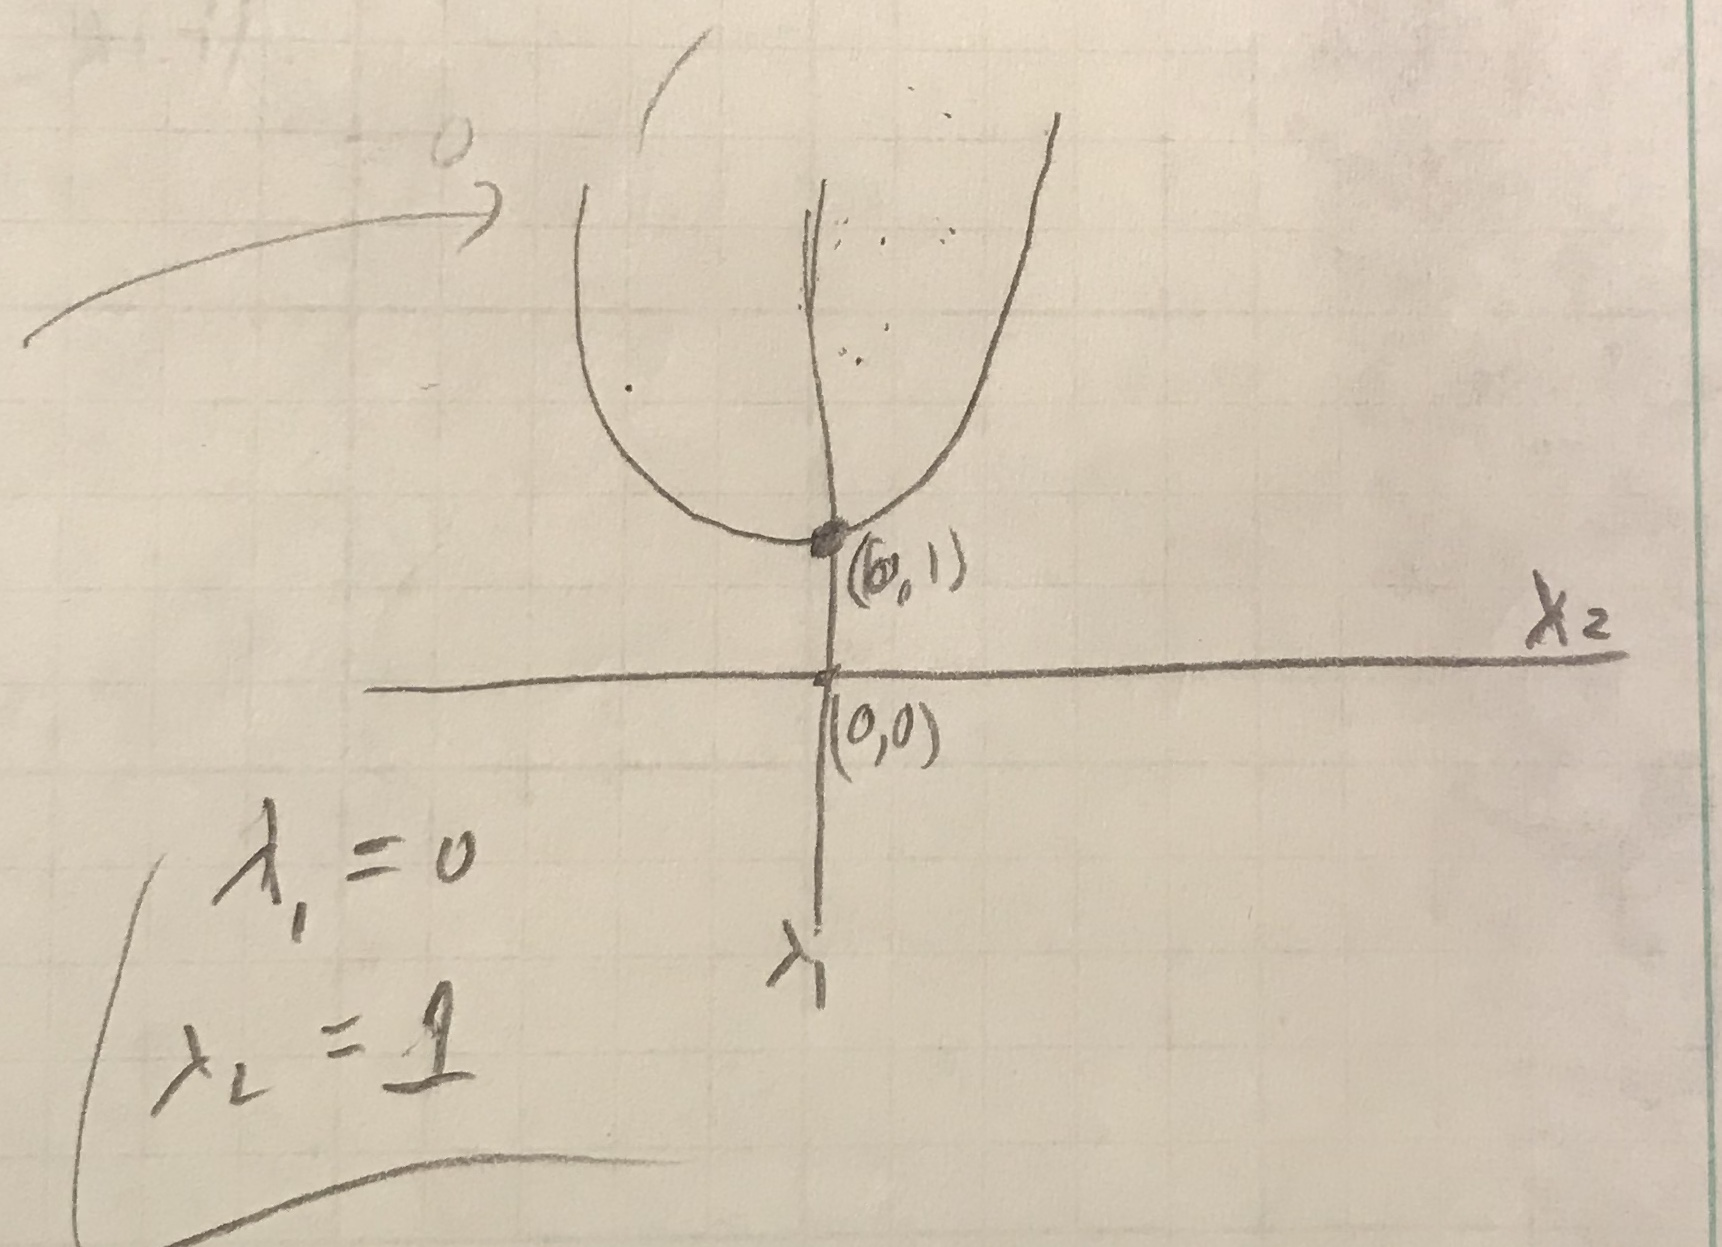
\includegraphics[width=\textwidth]{BSS4-4.jpeg}\\
We then have the following: 
    \begin{align*}
        &2x_1^2 -x_1x_2 + x_2^2 - 3x_1 + e^{2x_1 + x_2}\\
        &2(\bar x + \lambda d)^2 -(\bar x + \lambda d)(\bar x + \lambda d) + (\bar x + \lambda d)^2 - 3(\bar x + \lambda d)+ e^{2(\bar x + \lambda d) + (\bar x + \lambda d)}\\
        &2(\lambda d)^2 - 3\lambda  d + e^{3 \lambda d}\\
        &\text{Solving for } \lambda \\ 
        &2(\lambda)^2 - 3\lambda+ e^{3 \lambda}\\
        &\lambda_1 = 0\\
        &\lambda_2 = 1\\
    \end{align*}
d.) Dropping the last term from objective function:\\
    \begin{align*}
        &\min 2x_1^2 -x_1x_2 + x_2^2 - 3x_1\\
        &\nabla f(\bar x) = 
        \begin{bmatrix}
            4x_1 - x_2 -3\\
            -x_1 + 2x_2\\
        \end{bmatrix}
        = 
        \begin{bmatrix}
            0\\
            0\\
        \end{bmatrix}\\
        &\bar x_1 = 1/2 \bar x_2\\
        &4 \bar x_1 - 1/2 \bar x_1 - 3 = 0 \\ 
        &7/2\bar x_1 = 3
        &\bar x_1 = 6/7\\
        &\bar x_2 = 3/7\\
        &\bar = (6/7 , 3/7)\\ 
    \end{align*}
We then determine the $H(\bar x)$ matrix: 
    \begin{align*}
        &\nabla H(\bar x) = 
        \begin{bmatrix}
            4 & -1\\
            -1 & 2\\
        \end{bmatrix}\\
        &det|H(\bar x)| = 7 > 0 \quad H(\bar x) \text{is PD}\\
        &\min 2(6/7)^2 - (6/7)(3/7) + (3/7)^2 - 3 (6/7) = -9/7 
    \end{align*}
\section{BSS 4.7}
We consider the following problem:\\
\quad $\min (x_1 - 9/4)^2 + (x_2-2)^2$ \\
\quad s.t.\\
\quad $x_2 - x_1^2 \geq 0$\\
\quad $x_1 + x_2 \leq 6$\\
\quad $x_1 , x_2 \geq 0$\\
We reformulate the problem: \\ 
    \begin{align*}
        &\min (x_1 - 9/4)^2 + (x_2-2)^2\\
        &\text{s.t.} \\
        &x_1^2 - x_2 \leq 0\\
        &x_1 + x_2 \leq 0\\
        &-x_1 \leq 0\\
        &-x_2 \leq 0
    \end{align*}
a.) We find the following and adhere to the KKT conditions for $\bar x = (3/2 , 9/4) ^T$\\
    \begin{align*}
        &\nabla f(\bar x) + \sum_{i \in I} u_i \nabla g_i(\bar x) = 0\\
        &\nabla f(\bar x) = 
        \begin{bmatrix}
            (4x_1 - 9)/2\\
            2x_2 - 4\\
        \end{bmatrix}\\
        &\nabla f(\bar x) = 
         \begin{bmatrix}
            -3/2\\
            1/2\\
        \end{bmatrix} < 0 \\
        &\nabla g_1(\bar x) = 
         \begin{bmatrix}
            2x_1\\
            -1\\
        \end{bmatrix} = 
        \begin{bmatrix}
            3\\
            -1\\
        \end{bmatrix}\\
        &\nabla g_2(\bar x) = 
         \begin{bmatrix}
            1\\
            1\\
        \end{bmatrix}\\
        &\nabla g_3(\bar x) = 
         \begin{bmatrix}
            -1\\
            0\\
        \end{bmatrix}\\
        &\nabla g_4(\bar x) = 
         \begin{bmatrix}
            0\\
            -1\\
        \end{bmatrix}\\        
    \end{align*}
We then expand the KKT conditions: \\
    \begin{align*}
        &u_0 (-3/2 , 1/2)^T + u_1 (3, 1)^T + u_2 (1,1)^T + u_3(-1,0)^T + u_4(0,-1)^T = (0,0)^T\\
        &\text{We let } u_2=u_3 = u_4 = 0 \\
        &-3/2u_0 + 3u_1 = 0\\
        &u_1 = 1/2 u_0\\
        &1/2u_0 - u_1 = 0\\
        &u_1 = 1/2 u_0\\
        &\text{we let } u_0 = 1\\ 
        &u_0 = 1\\
        &u_1 = 1/2\\
        &u_2 = u_3 = u_4 = 0\\ 
        &u_i \geq 0
    \end{align*}
We find that $(3/2, 9/4)^T$ is  a KKT point.\\
b.) We then represent the condition graphically: \\ 
c.) We see that the objective function is convex, the constraints are convex. The feasible reagion is convex and identify that $(3/2, 9/4)^T$ is a KKT point. This adheres to the optimality and necessary conditions for KKT to demonstrate that $\bar x$ is local optimal solution and is a global optimal solution as well. \\
\section{BSS 4.13}
We have the following conditions for P and $\bar P$: We must write the KKT conditions for P and $\bar P$ and compare them. We will explain the difference between the 2.\\ 
    \begin{align*}
        &P: \quad \min f(x) \\
        &\text{s.t.}\\
        &g_i(x) \leq 0 \quad i = 1,...,m\\
        &h_j(x) = 0 \quad j = 1, ..., l\\ 
    \end{align*}
    \begin{align*}
        &\bar P \quad \min f(x) \\
        &\text{s.t.}\\
        &g_i(x) + s_i^2 = 0 \quad i = 1,...,m\\
        &h_j(x) = 0 \quad j = 1, ..., l\\ 
    \end{align*}
We assume that $f, g_i, and h_j$ are twice differentiable and that $X \subseteq R^n$ is nonempty open set and $S$ is the feasible set. We do the following relaxation and include the constraints within the objective function so that we can have a unconstrained minimizing problem.\\ 
    \begin{align*}
        &\phi(x, u, v) = f(x) + \sum_{i=1}^{m} u_i g_i(x) + \sum_{j=1}^{l} v_jh_j(x)\\
        &\text{We let $\bar x$ be a KKT Point for P and thus obtain \bar P}\\
        &\bar P:  \quad \min L(x) = \phi(x, \bar u, \bar v) = f(x) + \sum_{i=1}^{m} \bar u_i g_i(x) + \sum_{j=1}^{l} \bar v_j h_j(x)\\
        &x \in R^n
    \end{align*}
We find that the following conditions are true for $L(x)$: \\
    \begin{align*}
        &\sum_{i=1}^{m} \bar u_i g_i(x) \leq 0 \\
        &\sum_{j=1}^{l} \bar v_j h_j(x) = 0
    \end{align*}
Comparing both $P$ and $\bar P$ we see $P \leq  \bar P$\\
Thus we have $L(x) \leq f(x)$\\
We can then conclude that $L(\bar x) = f(\bar x)$. We have $\bar x$ as a local/global min for P,\\
    \begin{align*}
        &L(\bar x) \leq L(x) \quad x \in N_\epsilon (\bar x)\\
        &f(\bar x) = L(\bar x) \leq L(x) \leq f(x) \quad \forall x \in N_\epison (\bar x) \cap S\\
        &F \cap G_0'
    \end{align*}
\section{BSS 4.37}
We must consider the following problem: 
    \begin{align*}
        &\max x_1^2 + 4x_1x_2 + x_2^2\\
        &\text{s.t.}\\
        &x_1^2 + x_2^2 = 1
    \end{align*}
We reformulate the problem to obtain the primary minimizing problem:\\
    \begin{align*}
        &\min -x_1^2 - 4x_1x_2 - x_2^2\\
        &\text{s.t.}\\
        &-x_1^2 - x_2^2 = 1
    \end{align*}
a.) we find the KKT conditions for the minimizing reformulated problem:\\ 
    \begin{align*}
        &\nabla f(\bar x) = 
        \begin{bmatrix}
            -2x_1 - 4x_2 \\
            -4x_1 - 2x_2 \\
        \end{bmatrix} = 
        \begin{bmatrix}
            0 \\
            0 \\
        \end{bmatrix}\\
        &h_1 = 
        \begin{bmatrix}
            -2x_1 \\
            -2x_2 \\
        \end{bmatrix}
    \end{align*}
We identify 4 solutions to the problem:\\
    \begin{align*}
        &(1/\sqrt{2}, 1/\sqrt{2}), v = 3 \\ 
        &(-1/\sqrt{2}, -1/\sqrt{2}), v = 3 \\
        &(1/\sqrt{2}, 1/\sqrt{2}), v = -1 \\
        &(-1/\sqrt{2}, -1/\sqrt{2}), v = -1
    \end{align*}
We must consider constraint qualification (CQ) and determine that the KKT conditions are necessary for optimality.\\ 
    \begin{align*}
        &\bar x_1 = (1/\sqrt{2} ,1/\sqrt{2}) \\
        &\bar x_2 = (-1/\sqrt{2} ,-1/\sqrt{2})
    \end{align*}
b.)We will test for the second order optimality conditions: \\
We define L(x): \\
    \begin{align*}
        &L(x) = -x_1 - 4x-1x_2 - x_2^2 + v (-x_1^2 - x_2^2 -1)\\
        &\nabla^2 L(x) = 2
        \begin{bmatrix}
            v- 1 & -2 \\
            -2 & v-1\\ 
        \end{bmatrix}
    \end{align*}
We can only find the second order optimality true when $v = 3$  and have $\nabla^2 L(x)$ as Positive Definite (PD). 
c.) The unique optimal solution is found and demonstrated utilizing the KKT conditions and first and second order conditions for optimality thus finding the following as strict local optima.
    \begin{align*}
        &\bar x = (1/\sqrt{2}, 1/\sqrt{2}), v = 3 \\ 
        &\bar x = (-1/\sqrt{2}, -1/\sqrt{2}), v = 3
    \end{align*}
\section{BSS 4.39} 
We consider the following problem:\\
    \begin{align*}
        &\max \quad (x_1 -2)^2 + (x_2 - 3)^2\\
        &\text{s.t.}\\
        &3x_1 + 2x_2 \geq 6\\
        &-x_1 + x_2 \leq 3\\
        & x_1 \leq 2
    \end{align*}
We reformulate the problem to the primal so that we can minimize and determine optima: \\ 
    \begin{align*}
        &\min \quad -(x_1-2)^2 - (x_2-3)^2 \\
        &\text{s.t.}\\
        & -3x_1 - 2x_2 \leq 6 \\ 
        & x_1 - x_2 \geq 3\\
        &-x_1 \geq 2
    \end{align*}
We graphically represent the local min solns: \\
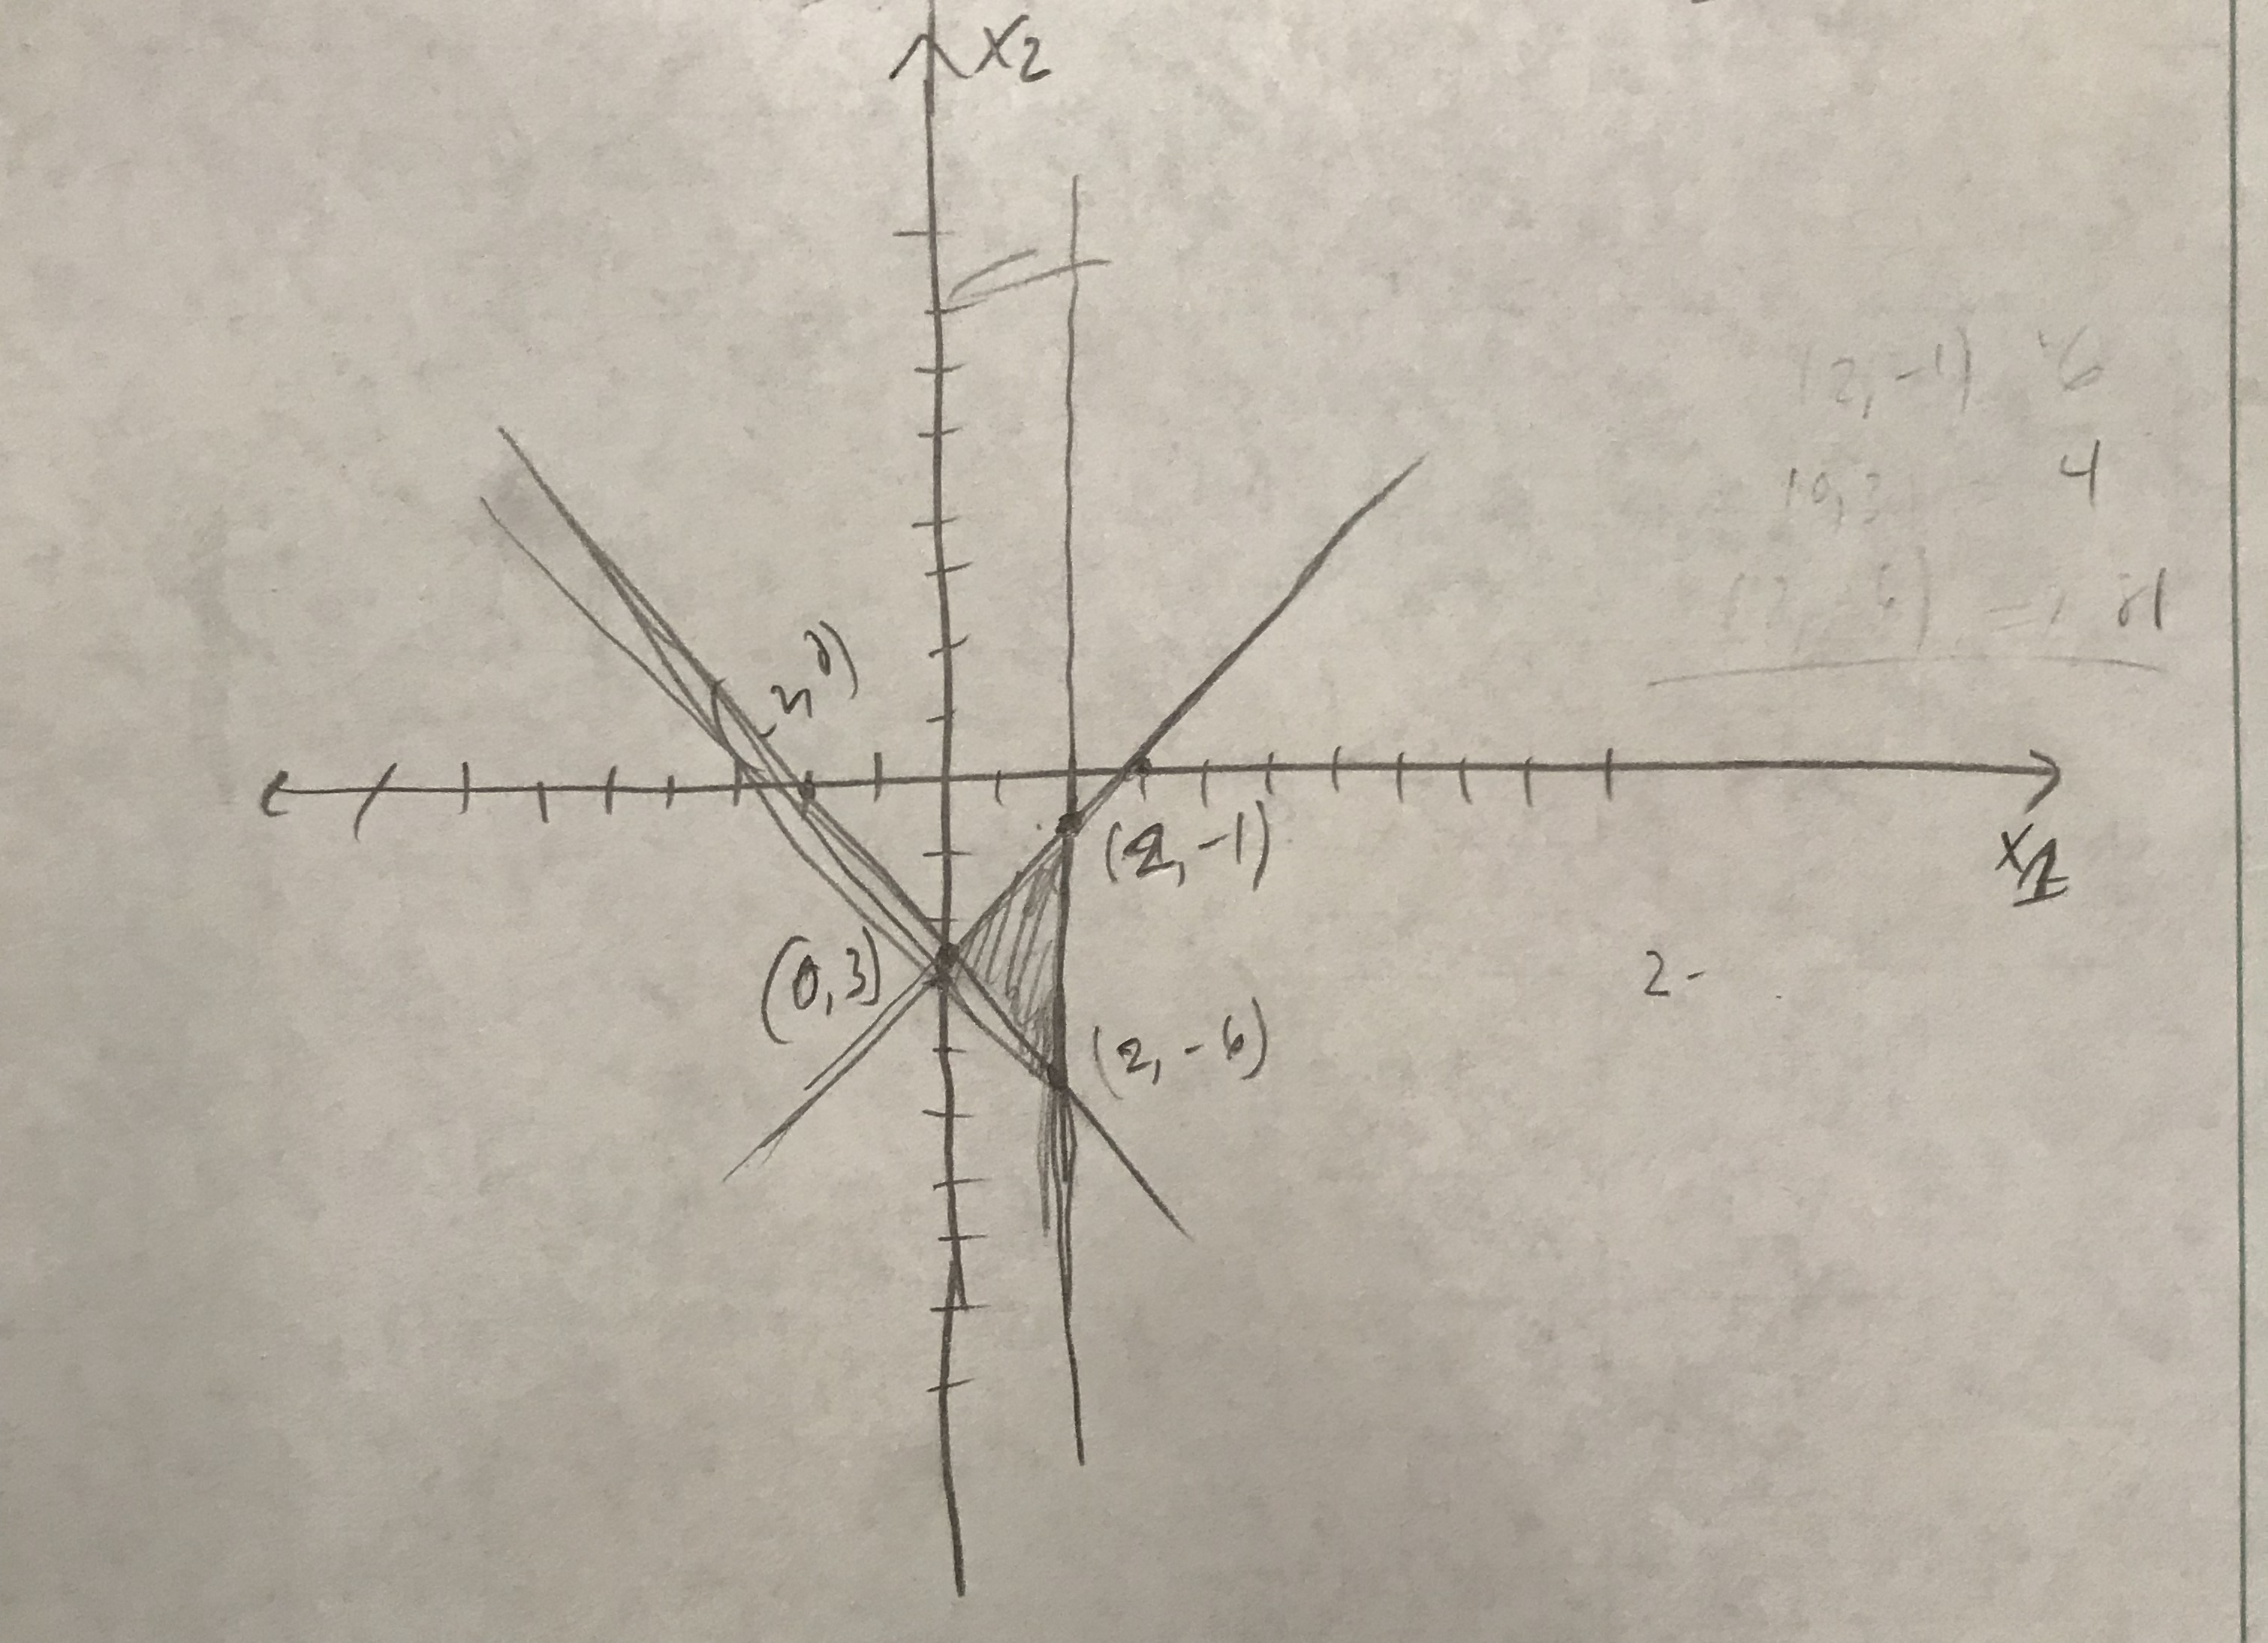
\includegraphics[width=\textwidth]{BSS4-39.jpeg}\\
We get the global maximum to be 81 with extreme point $\bar x = (2 , -6) $\\ \\
b.) We utilize first and second order KKT optimality characterization:\\
    \begin{align*}
        &L(x) = -x_1^2 + 4x_1 - 4 -x_2^2 + 6x_2 -9 + u_1 (-3x_1 -2x_2 - 6) + u_2 (x_1 -x_2 -3) + u_3 (-x_1 -2)\\
        &\nabla L(\bar x) =
        \begin{bmatrix}
            -2x_1 + 4 - 3u_1 + u_2 - u_3 \\
            -2x_2 + 6 -2u_1 - u_2\\
        \end{bmatrix} =
        \begin{bmatrix}
            0\\
            0\\
        \end{bmatrix}
    \end{align*}
    We determine $\nabla^2 L(\bar x)$:\\
    \begin{align*}
        &\nabla^2 L(\bar x) = 
        \begin{bmatrix}
            -2 & 0\\
            0 & -2\\
        \end{bmatrix}\\
        &det|\nabla^2 L(\bar x) | = 4 - 0 = 4 > 0
    \end{align*}
Because of the first and second order KKT conditions we determine a strict local min for problem. 
\end{document}